\chapter{Experimental Results} \label{chap:experimental-results}
This chapter presents the experimental results obtained during the customization, debugging and verification of the ORB-SLAM algorithm for edge computing and the use of the methodology for ROS-based robotics application based on Docker and Kubernetes.
First the chapter describes the Hardware and Software setup used during the experiments. Then, it explains how the presented methodology has been applied to merge ORB-SLAM and a typical robotic system developed for mobile robot navigation in a warehouse scenario.

The main technical specifications of the \textit{Host} and the embedded device used during the experiments are shown in table \ref{tab:tech-specs-host} and in table \ref{tab:tech-specs-tx2} respectively. 

\begin{table}[htbp]
	\centering
	\begin{tabularx}{\linewidth}{|l|X|}
		\hline
		\rowcolor{Gray}
		Hardware         & Model \\
		\hline
		Processor        & Intel(R) Core(TM) i5-7400 CPU @ 3.00GHz \\
		Storage          & SATA 500GiB \\
		Memory           & 16GiB \\
		GPU              & NVIDIA GeForce GTX 980 \\
		\hline
		\rowcolor{Gray}
		Software         & Version \\
		\hline
		Operating System & Ubuntu 18.04 \\
		OpenCV           & 3.4.7 \\
		CUDA             & 10.0 \\
		ROS              & Melodic Moreina \\
		\hline
	\end{tabularx}
	\caption{Technical specifications of the Host \label{tab:tech-specs-host}}
\end{table}

\begin{table}[htbp]
	\centering
	\begin{tabularx}{\linewidth}{|l|X|}
		\hline
		\rowcolor{Gray}
		Hardware         & Model \\
		\hline
		Processor        & Dual-core Denver 2 64-bit CPU and quad-core ARM A57 complex \\
		Storage          & eMMC 5.1 32 GB \\
		Memory           & LPDDR4 8 GB 128-bit \\
		GPU              & NVIDIA Pascal™ architecture with 256 NVIDIA CUDA cores 1.3 TFLOPS (FP16) \\
		\hline
		\rowcolor{Gray}
		Software         & Version \\
		\hline
		Operating System & 18.04.1-Ubuntu \\
		OpenCV           & 3.4.7 \\
		CUDA             & 10.0  \\
		ROS              & Melodic Moreina \\
		\hline
	\end{tabularx}
	\caption{Technical specifications of NVIDIA Jetson TX2. \label{tab:tech-specs-tx2}}
\end{table}


\section{Mobile robots application}


\subsection{Architecture at L1}
At this architecture level we put a whole ROS-based system on a single Intel x86 powered machine that we will conventionally call \textit{Host}.
As shown in figure \ref{fig:l1archexp}, in this case there are two main ROS nodes that communicate: the ORB-SLAM2, described in chapter \ref{chap:verification}, and a hybrid motion planner (VOVD \cite{VOVD}). Both applications act as ROS nodes to perform a mobile robot 2D navigation task.

\begin{figure}[htbp]
	\centering
	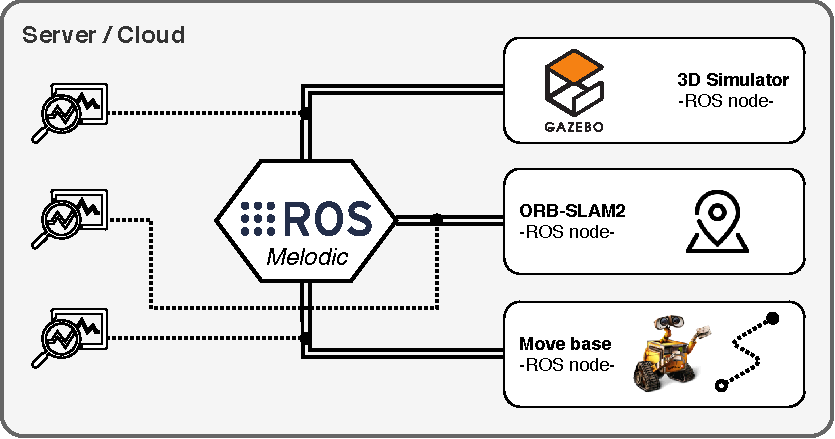
\includegraphics[width=\textwidth]{images/L1-arch-exp}
	\caption{L1 architecture used during the experiments}
	\label{fig:l1archexp}
\end{figure}

Because of the most used robotics platforms used today support the Melodic Morenia \cite{rosmelodic} version of ROS, and because VOVD was written with the Kinetic version, it has been decided to convert VOVD in the relative Melodic ROS version. This task required a redefinition of some functions related to the ROS \mintinline{cpp}{tf2} package \cite{tfros} due to the deprecation of the \mintinline{cpp}{tf} package functions previously used. 
Another modification done is related to the 3D map used by Gazebo \cite{Gazebo} simulator. The problem was that it came with a featureless map generated from an ``.pgm'' file (see fig. \ref{fig:mapfile}), and because of ORB-SLAM2 properly works only if some features are detected during its execution, it has been necessary to add a material to the 3D model of the map. The results obtained before and after applying the material on the 3D map are visible in figure \ref{fig:3Dmapcomparison}.

\begin{figure}[htbp]
	\centering
	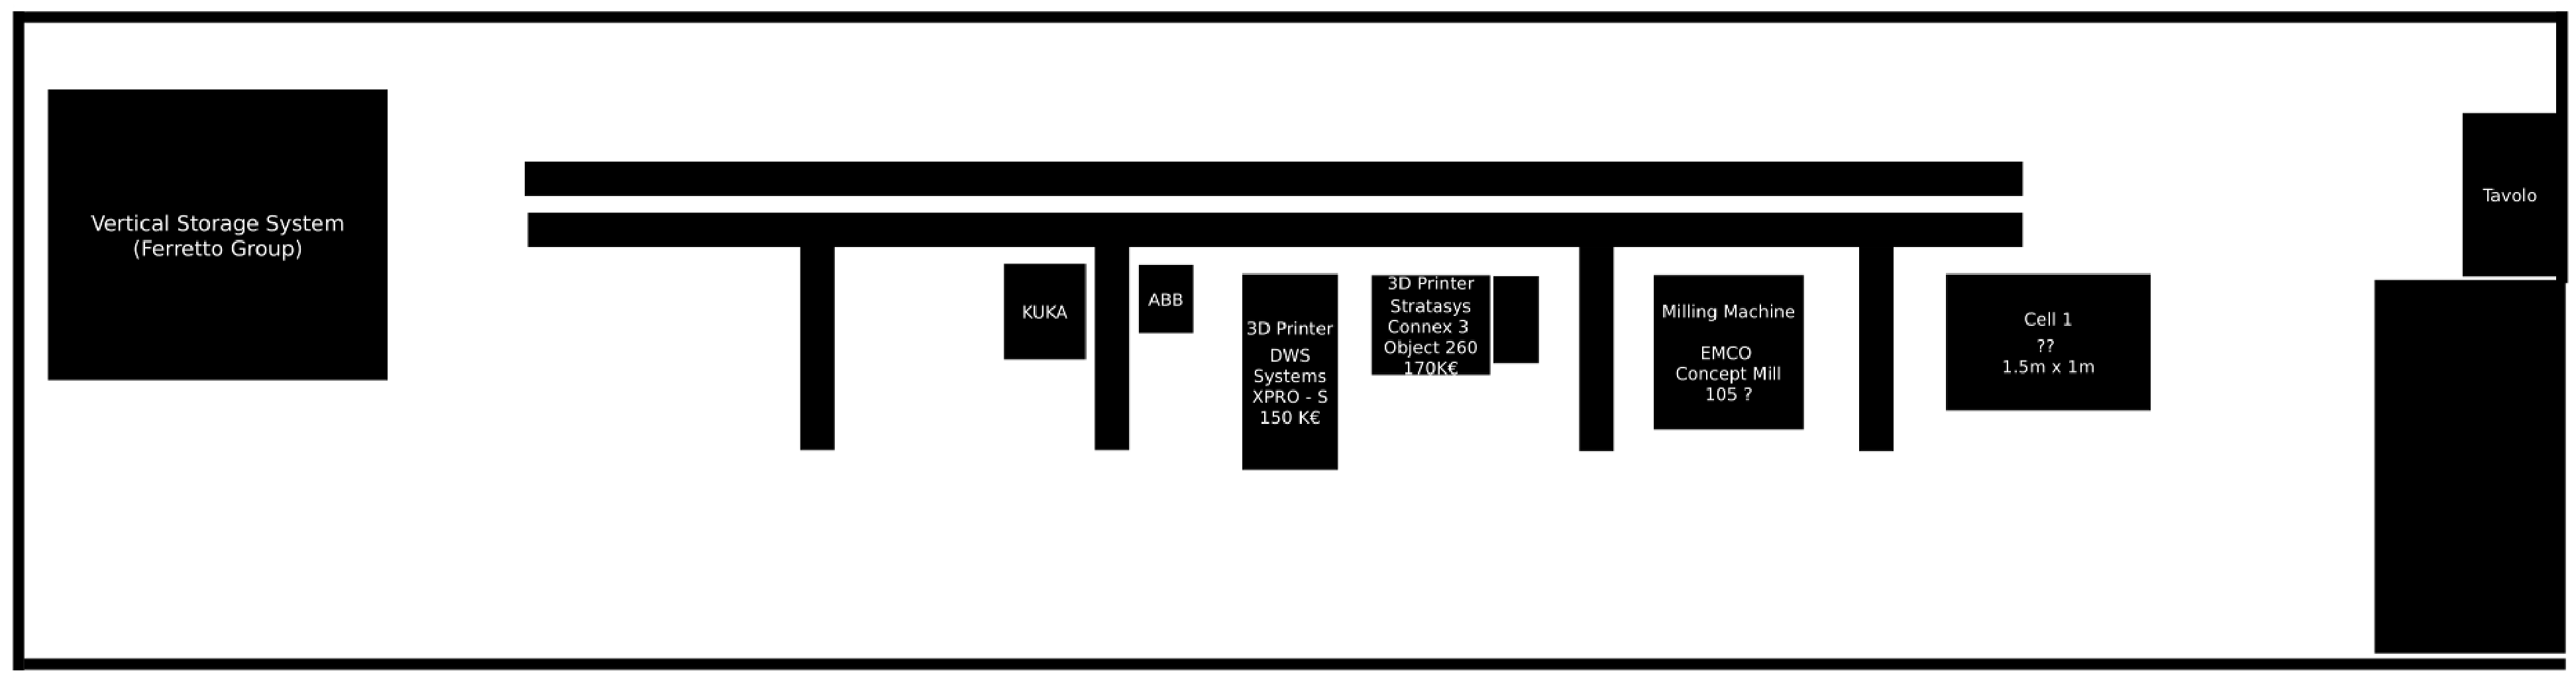
\includegraphics[width=\textwidth]{images/icelabmap}
	\caption{pgm file map description of IceLab.}
	\label{fig:mapfile}
\end{figure}

Talking about ORB-SLAM2, it comes already provided with the necessaries functions to run in a ROS environment, thus no others operations have been required to complete the first architecture level.
	
\begin{figure*}[htbp]
	\centering
	\subfloat[Map with material    \label{fig_first_case}]{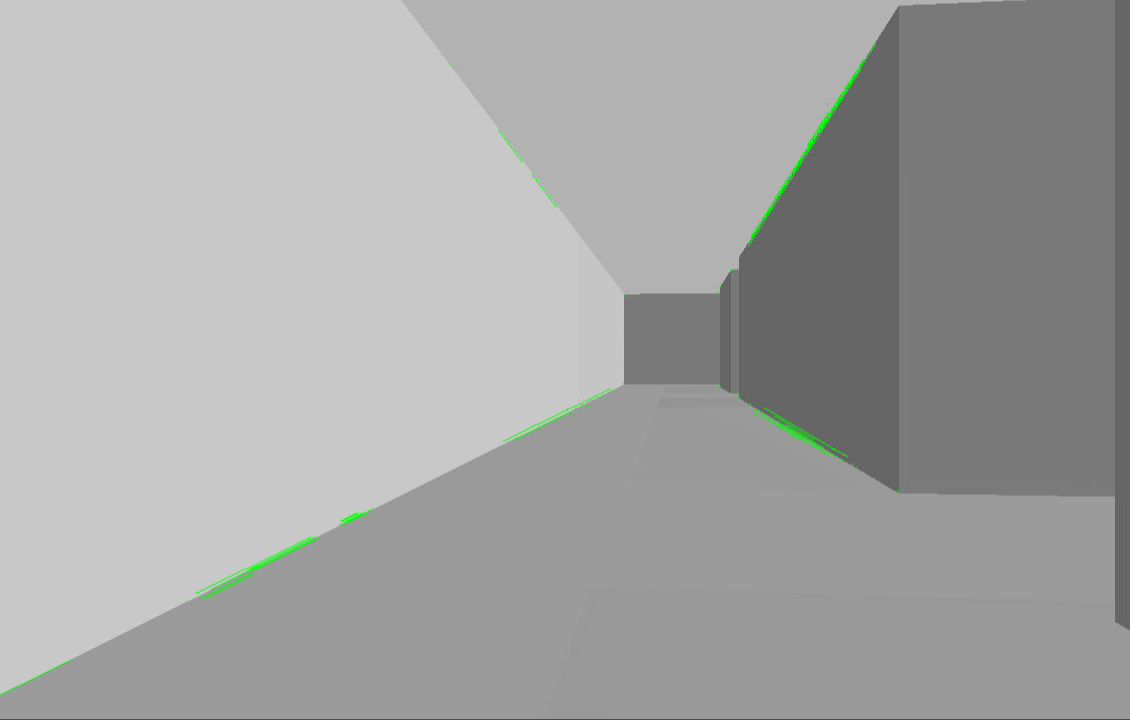
\includegraphics[width=2.4in]{images/orb-featureless-ed.png}}
	\hfil
	\subfloat[Map without material   \label{fig_second_case}]{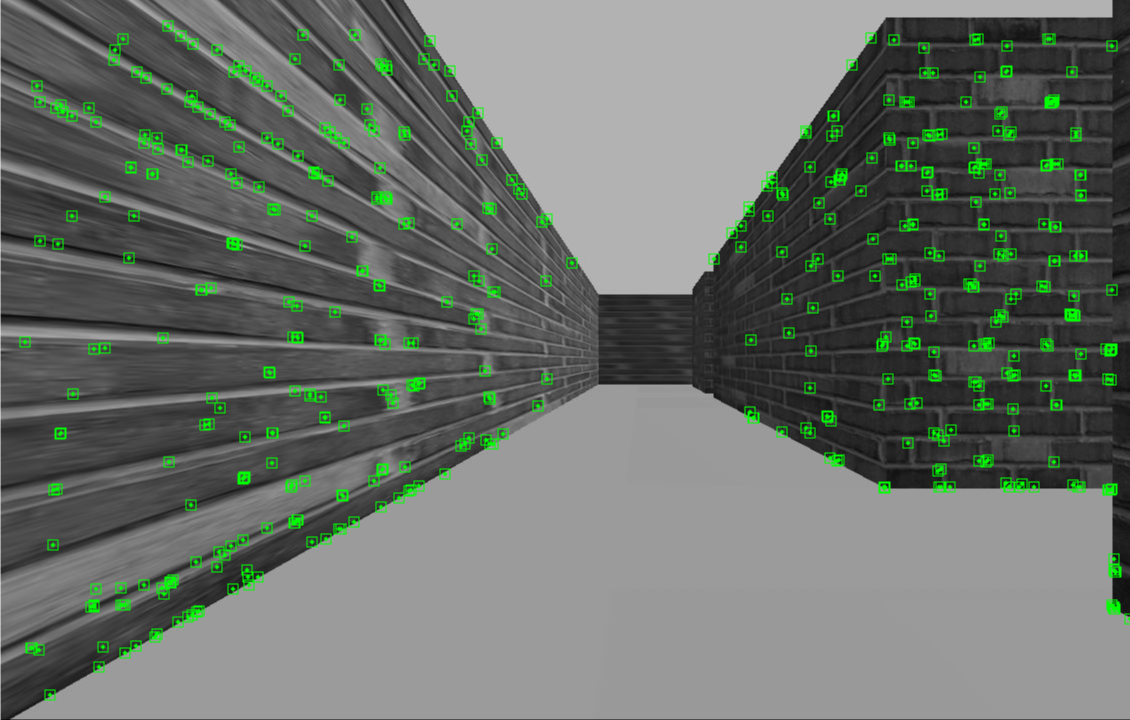
\includegraphics[width=2.4in]{images/orb-features-ed.png}}
	%
	\caption{3D maps material comparison}
	\label{fig:3Dmapcomparison}
\end{figure*}

Thanks to the modularity of ROS we were able to verify the functional behaviour of the system implementing  a custom ROS node that acts as a monitor. It listens on all topics of the system and captures the informations of interest.  
To obtain a more accurate performance measurement, we added some time points within the source code of both VOVD and ORB-SLAM2. Specifically speaking for VOVD we measure the time to perform the local planner computation. To the ORB-SLAM2 side instead we measure the time to elaborate each frame coming from the simulator camera.
The performance measurement obtained at this architecture level are shown in table \ref{tab:resultL1-exp}.

\begin{table}[htbp]
	\begin{tabularx}{\linewidth}{@{}l*{7}{C}c@{}}
		\toprule
		\hline
		Setup              & Odom (ms) & Track Pipe (ms) & Frame Elab. (ms) & Feature Ext.(ms) & Supp. (FPS) \\
		\hline
		orbslam            & -             & 18.52          & 24.09                 & 22.04                  & 41.45      \\ \hline
		vovd           	   & 1.20          & -              & -                     & -                      & -          \\ \hline
		(orb;vovd)     	   & 2.33          & 38.99          & 39.93                 & 36.75                  & 25.03      \\ \hline
		\bottomrule
	\end{tabularx}
	\caption{\label{tab:resultL1-exp}Performance measurement at L1 architecture.}
\end{table}

\subsection{Architecture at L2}
Another common architecture in robotics involves the distribution of ROS nodes on different hardware platforms. In our case we have two NVIDIA Jetson TX2. 
This step requires the split of our system in two parts: the \textit{Host}, on which runs Gazebo simulator, and the \textit{Device/s} that will perform either the robot navigation and SLAM.
Figure \ref{fig:l2arch-exp} shows the configuration we setup during the experiment.

\begin{figure}[htbp]
	\centering
	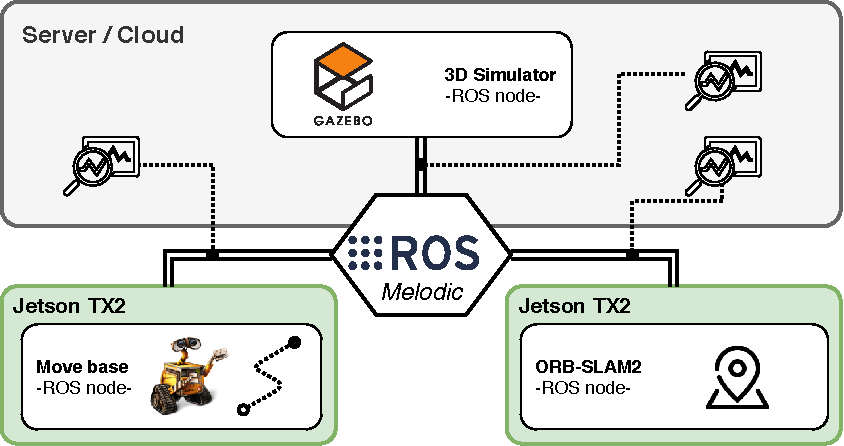
\includegraphics[width=\textwidth]{images/L2-arch-exp}
	\caption{L2 architecture used during the experiments}
	\label{fig:l2arch-exp}
\end{figure}

Due to the several interconnected nodes, each of which having many parameters, it is recommanded to create a roslaunch file  using the \textit{machine tag}. As explained in chapter \ref{chap:methodology}, these tags allow to control on which machines the node run.

At this architecture level the main focus is on the communication between the \textit{Host}, that acts as Master, and the other external nodes that represent the slaves. It is important to verify that the system continues working properly and that the Network doesn't become a bottleneck. For example, if we need to transfer a stream of images from one ROS node to another that is running on different machine, we should compress each frame before send it over the network. In this way, we avoid to saturate the bandwidth of the network. In our case the compression task is performed to the Host side from the robot's camera within Gazebo simulator. The decompression instead is computed on Jetson by the ORB-SLAM2 node whenever it receives a new frame to elaborate.
We measured the performance of the system in the same way we have done in the previous architecture level.
Note that, as expected, the performance of ORB-SLAM2 are dropped down due to the limited computing capability of the Jetson. This is more highlighted when we run both VOVD and ORB-SLAM2 on the same device because they are competing for the hardware resources.
The new performance measurements are presented in table \ref{tab:resultL2-exp}.
Note that, due to the modularity of ROS, we were able to fine tune the system without making any change to the code. For example, we can easily modify either frequency of the camera output or the number of key-points extracted for each incoming frame.
Another parameter to consider is the bandwidth of the network. The virtual Asus Xtion camera used by Gazebo publish images with a resolution of 1280*720*3 at 20 frames per second.
Computers hooked up to LANs are connected using Cat5 cable. Although the Cat5 ethernet cable can handle up to 10/100 Mbps at a 100 MHz bandwidth, it is not sufficient to transfer the data coming from the camera because it requires a bandwidth of 442 Mps.
This is the reason why we measured the data decompression time performed by the ORB-SLAM2 ROS node.

\begin{table}[htbp]
	\begin{tabularx}{\linewidth}{@{}l*{7}{C}c@{}}
		\toprule
		\hline
		Setup              & Odom (ms) & Track Pipe (ms) & Dec. (ms) & Frame Elab. (ms) & Feature Ext.(ms) & Supp. (FPS) \\
		\hline
		\rowcolor{Gray}
		\multicolumn{7}{c}{Performance Measurement: camera 10 Hz}                                                                                                                                           \\
		\hline
		orb(j1)            & -             & 43.41          & 13.08             & 49.21                 & 43.62                  & 20.32           \\ \hline
		vovd(j1)           & 1.70          & -              & -                 & -                     & -                      & -               \\ \hline
		(orb;vovd)(j1)     & 2.58          & 73.49          & 18.69             & 62.70                 & 54.76                  & 13.61           \\ \hline
		(orb(j1);vovd(j2)) & 1.60          & 49.81          & 13.53             & 49.25                 & 43.01                  & 20.08           \\ \hline
		\rowcolor{Gray}
		\multicolumn{7}{c}{Performance Measurement: camera 20 Hz}                                                                                                                                           \\
		\hline
		orb(j1)            & -             & 54.82          & 14.47             & 49.40                 & 44.35                  & 18.24           \\ \hline
		vovd(j1)           & 1.70          & -              & -                 & -                     & -                      & -               \\ \hline
		(orb;vovd)(j1)     & 2.85          & 93.15          & 23.96             & 67.99                 & 60.41                  & 10.74           \\ \hline
		(orb(j1);vovd(j2)) & 1.60          & 56.20          & 14.00             & 49.32                 & 43.95                  & 17.79           \\ \hline
		\bottomrule
	\end{tabularx}
	\caption{\label{tab:resultL2-exp}Performance measurement at L2 architecture.}
\end{table}



\subsection{Architecture at L3}
Finally we reached the last architecture level of the design flow. It is composed by the \textit{Host}, \textit{Device/s } and the real robot \textit{Robot/s}. In our case the real robot is the KUKA YouBot \cite{YouBot} provided by the robotics laboratory ALTAIR  from University of Verona.

The key point here is that if the simulator has been properly configured at L1 architecture (as described in chapter \ref{chap:methodology}),  the operation to detach the simulator and attach back the real robot is completely transparent with respect to the entire system. This is one of the main advantage we had benefit due to the modularity of ROS.

As we can see in Fig. \ref{fig:l3archexp}, the simulator has been removed from the \textit{Host} and it has been replaced by the real robot, on which one or more embedded devices can be attached.

\begin{figure}[tbp]
	\centering
	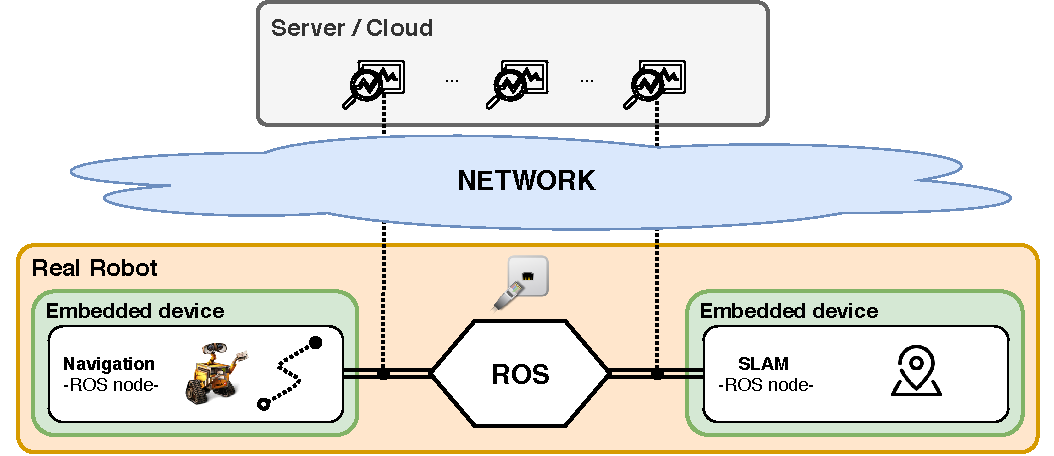
\includegraphics[width=\textwidth]{images/L3-arch-exp}
	\caption{L3 architecture}
	\label{fig:l3archexp}
\end{figure}


\section{Deployment from the cloud to the edge}
This section describes the process used in the project to prepare both VOVD and ORB-SLAM2 applications for the edge computing through the support of KubeEdge.
As mentioned in section \ref{sec:kubeedgebackground}, KubeEdge is built upon Kubernetes and provides fundamental infrastructure support for network, application deployment and metadata synchronization between cloud and edge. As we know, Kubernetes uses containers to run isolated, packaged applications across its cluster nodes. To run on Kubernetes, our applications must be encapsulated in one or more container images and executed using a container runtime like Docker. While containerizing components is a requirement for Kubernetes, it also allows for scaling and management. For instance, containers provide isolation between the application environment and the external host system, support a networked, service-oriented approach to inter-application communication, and typically take configuration through environmental variables and expose logs written to standard error and standard output. Containers themselves encourage process-based concurrency and help maintain dev/prod parity by being independently scalable and bundling the process's runtime environment. These characteristics made possible to package our applications so that they run smoothly on Kubernetes.


\subsection{Dockerization}
At this point the main goal of the project was to reach the edge devices from the host/cloud server wherever they are.
For this purpose, at firt we needed to containerize both VOVD and ORB-SLAM2 for NVIDIA Jetsons.
Since both are wrapped as ROS nodes, we had to include the ROS (Melodic) base distro and the required dependencies to run our applications.
Listing \ref{lst:dockerfilevovd} shows the Dockerfile used to containerize VOVD during the experiments.

\begin{listing}[htbp]
	\begin{minted}[
	framesep=2mm,
	baselinestretch=1.2,
	fontsize=\footnotesize,
	linenos,
	breaklines
	]{bash}
	FROM ros:melodic-ros-base
	
	# set args
	ARG ip=192.168.254.3
	ARG master_uri=http://192.168.254.2:11311
	
	# set enviroment
	ENV ROS_MASTER_URI=$master_uri ROS_IP=$ip ROS_WS=/home/catkin_ws
	
	COPY VOVD install_dependencies.sh ./
	
	# install ros packages
	RUN mkdir -p $ROS_WS/src && mv VOVD $ROS_WS/src && \
	chmod +x install_dependencies.sh && sh install_dependencies.sh && \
	. "/opt/ros/$ROS_DISTRO/setup.sh" && cd $ROS_WS && catkin_make && \
	sed --in-place --expression '$isource "$ROS_WS/devel/setup.bash"' \
	/ros_entrypoint.sh
	
	# set the working directory
	WORKDIR $ROS_WS
	
	# run ros package launch file
	ENTRYPOINT ["roslaunch", "vo_controller"]
	CMD ["test_edge.launch"]
	\end{minted}
	\caption{Dockerfile used to create the Docker image of VOVD.}
	\label{lst:dockerfilevovd}
\end{listing}

In phase of image's building we set the \mintinline{bash}{--network=host} flag in order to enable the communication over the ROS network among containers running on different machines.
This is all about the containerization of a ``simple'' ROS node such as VOVD.

To the other side ORB-SLAM2 also needs to access to the GPU of the device.
On NVIDIA NGC web portal, Linux4Tegra (L4T) package provides the bootloader, kernel, necessary firmwares, NVIDIA drivers, flashing utilities and a sample filesystem to be used on Jetson systems. The software packages contained in L4T provide the functionality necessary to run Linux on Jetson devices (Xavier, TX2, and Nano).
Thus in this case the L4t image provided by NVIDIA is a more affordable starting point for the containerization of the ORB-SLAM2.
Furthermore we know that ORB-SLAM2 is an heterogeneous application made of a wide variety of libraries such OpenCV, OpenVX, CUDA, TensorRT and so on.
Consequently we had to provide all of these libraries within the dockerfile in order to build our application.

%TODO Problemi in fase di building del container --> ROS + GPU (TRT)
%One of the problem we faced during this operation is related to the storage of the Jetson TX2.  Lo diciamo??



\section{The whole system on KubeEdge}
After a functional verification at container's level, the system is almost ready to be deployed from the cloud to the edge using kubeEdge.
Following the procedure described in section \ref{sec:deployment}, first we setup our cluster in order to enable the physical and virtual communication between the Host (to the cloudside) and edge nodes (to the edgeside).
Then we created three configuration files for each application we want to deploy to the edge.
These configuration files contain the informations for device model, device instance and deployment respectively.

%TODO qui si potrebbe dire di più ad esempio come abbiamo configurato host e jetson i file di device model device instance e deployment
During our experiments we tested the system in various conditions: we forced the deployment either to a single device or across multiple devices.
The performance measurements done with the system running on KubeEdge are shown in table \ref{tab:resultL3-exp}.
The results show that KubeEdge platform does not contribute to the normal network latency in a significant way (the container image download time is not included in the test).




\begin{table}[htbp]
	\begin{tabularx}{\linewidth}{@{}l*{7}{C}c@{}}
		\toprule
		\hline
		Setup              & Odom (ms) & Track Pipe (ms) & Dec. (ms) & Frame Elab. (ms) & Feature Ext.(ms) & Supp. (FPS) \\
		\hline
		\rowcolor{Gray}
		\multicolumn{7}{c}{KubeEdge - Performance Measurement: camera 10 Hz}                                                                                                                                           \\
		\hline
		orb(j1)            & -             & 47.28          & 12.78             & 40.52                 & 36.02                  & 21.15           \\ \hline
		vovd(j1)           & 1.30          & -              & -                 & -                     & -                      & -               \\ \hline
		(orb;vovd)(j1)     & 1.40          & 82.47          & 15.10             & 53.54                 & 48.09                  & 12.12           \\ \hline
		(orb(j1);vovd(j2)) & 1.38          & 50.83          & 13.98             & 43.80                 & 38.04                  & 19.67           \\ \hline
		\rowcolor{Gray}
		\multicolumn{7}{c}{KubeEdge - Performance Measurement: camera 20 Hz}                                                                                                                                           \\
		\hline
		orb(j1)            & -             & 50.20          & 16.20             & 42.16                 & 34.82                  & 19.92           \\ \hline
		vovd(j1)           & 1.21          & -              & -                 & -                     & -                      & -               \\ \hline
		(orb;vovd)(j1)     & 1.43          & 70.54          & 15.02             & 55.60                 & 50.24                  & 14.18           \\ \hline
		(orb(j1);vovd(j2)) & 1.26          & 58.14          & 13.52             & 42.34                 & 37.17                  & 17.20           \\ \hline
		\bottomrule
	\end{tabularx}
	\caption{\label{tab:resultL3-exp}}
\end{table}



%%%%%%%%%%%%%%%%%%%%%%5
\clearpage
\thispagestyle{empty}